% Distributed under the Apache license, Version v2.0
% Copyright 2019 Felipe Estrada-Solano <festradasolano at gmail>
% Based on Keith A. Gillow's OCIAM Thesis lyx files
% ==============
% DOCUMENT CLASS
% ==============
%\documentclass[11pt,draft]{thesis_proposal-fiet_unicauca} % draft version
\documentclass[11pt,twoside]{thesis_proposal-fiet_unicauca} % submission version
% ==============
% LaTeX PACKAGES
% ==============
% -----
% Color
\usepackage{xcolor}
% -----
% Fonts
\usepackage{lmodern}
\usepackage{helvet}
\renewcommand{\familydefault}{\sfdefault}
\usepackage[utf8]{inputenc}
% -----------
% Other fonts
\usepackage{listings}
\usepackage{verbatim}
% ---------
% Page size
\usepackage[letterpaper]{geometry}
\geometry{verbose,tmargin=3cm,bmargin=2.5cm,lmargin=3cm,rmargin=2.5cm,headheight=3cm,headsep=1cm}
% -----------
% Hyphenation
\usepackage[american]{babel}
% \usepackage[spanish]{babel}
% -------------
% Table columns
\usepackage{array}
% -------------
% External PDFs
\usepackage{pdfpages}
% -------------
% Math formulas
\usepackage{amsmath}
\usepackage{amssymb}
% --------
% Graphics
\usepackage{graphicx}
\graphicspath{{figures/}} % path(s)
%\DeclareGraphicsExtensions{.eps} % extension(s)
% ------------
% Bibliography
\usepackage[numbers]{natbib}
% ------------
% Period label separation instead of colon
\usepackage[labelsep=period]{caption}
% ----------------
% Hyper-references

% Draft-version
\usepackage[unicode=true, bookmarks=true, bookmarksnumbered=true, bookmarksopen=false, breaklinks=true, pdfborder={0 0 0}, backref=page, colorlinks=true]{hyperref}

% Submission-version
% \usepackage[unicode=true, bookmarks=true, bookmarksnumbered=true, bookmarksopen=false, breaklinks=true, pdfborder={0 0 0}, colorlinks=true]{hyperref}
% ----------------
% Table formatting
\usepackage{array}
\usepackage{multirow}
\usepackage{makecell}
% ---------------
% List formatting
\usepackage{enumitem}
% --------------
% Text alignment
\usepackage{ragged2e}
% ----------------
% Graphic elements
\usepackage{tikz}
% -------------
% Gantt diagram
\usepackage{gantt}
% ---
% URL
\usepackage{url}
% ===============
% LaTeX UTILITIES
% ===============
% ----------------
% Hyper-references

% Digital-version
\hypersetup{pdftitle={Title of the Thesis}, pdfauthor={Name of the Student}, colorlinks=true, citecolor=blue, linkcolor=blue, urlcolor=blue}

% Print-version
% \hypersetup{pdftitle={Title of the Thesis}, pdfauthor={Name of the Student}, colorlinks=false}
% ----------------
% Grayscale colors
\definecolor{light-gray}{gray}{0.90}
\definecolor{medium-light-gray}{gray}{0.70}
\definecolor{medium-dark-gray}{gray}{0.40}
\definecolor{dark-gray}{gray}{0.20}
% ---------------------------------------------------------------
% Pages with more than 80% of floats become pure float-only pages
\renewcommand{\floatpagefraction}{.8}%
% -----------------------
% Extra height for tables
\renewcommand{\arraystretch}{1.6}
% -------------
% Abbreviations
\newcommand{\etal}{\textit{et al.} }
\newcommand{\cf}{\textit{cf.}, }
\newcommand{\eg}{\textit{e.g.}, }
\newcommand{\ie}{\textit{i.e.}, }
\newcommand{\etc}{\textit{etc}.}
\newcommand{\wrt}{\textit{w.r.t.} }
% ------------------------------
% Center text of cells in tables
\newcommand{\centertext}[1]{\hspace*{\fill}#1\hspace*{\fill}}
% ------------------
% Same font for URLs
\urlstyle{same}
% ----------------
% URL break styles
\makeatletter
\def\url@allbreakstyle{%
  \def\UrlBreaks{\do\.\do\@\do\\\do\/\do\!\do\_\do\|\do\;\do\>\do\]%
    \do\)\do\,\do\?\do\'\do+\do\=\do\#%
    \do A\do B\do C\do D\do E\do F\do G\do H\do I\do J\do K\do L\do M%
    \do N\do O\do P\do Q\do R\do S\do T\do U\do V\do W\do X\do Y\do Z%
    \do a\do b\do c\do d\do e\do f\do g\do h\do i\do j\do k\do l\do m%
    \do n\do o\do p\do q\do r\do s\do t\do u\do v\do w\do x\do y\do z%
    \do 0\do 1\do 2\do 3\do 4\do 5\do 6\do 7\do 8\do 9%
  }%
}
\def\url@restrictedbreakstyle{%
  \def\UrlBreaks{\do\.\do\@\do\\\do\/\do\!\do\_\do\|\do\;\do\>\do\]%
    \do\)\do\,\do\?\do\'\do+\do\=\do\#}%
}
\makeatother
% ----------------------
% Define URL break style
\urlstyle{allbreak}
% \urlstyle{restrictedbreakstyle}
% ==================
% DOCUMENT UTILITIES
% ==================
% -------------
% Unicauca logo
\def\logo{{
\includegraphics[scale=0.45]{logo_unicauca.pdf}}}
% ---------------------------------------
% Arguments for the cover and title pages

% Title of the thesis or capstone project
\title{Title of the Thesis/Project}
% Full name of the student
\author{Name of the Student}
% Name of the thesis degree (e.g., Master's, Ph.D.)
\degree{Master's/Ph.D.}
% Name of the program without degree
\program{Program}
% Full name of the advisor
\advisor{Name of the Advisor}
% Abbreviated advisor's degree (e.g., M.Sc., Ph.D.)
\advisordegree{M.Sc./Ph.D.}
% Name of the line of research
\lineresearch{Name of the Line of Research}
% Submission month of the proposal
\submitmonth{Month}
% Submission year of the proposal
\submityear{Year}

% Full name of the co-advisor (if no co-advisor, do not comment, just define \coadvisor as empty)
\coadvisor{Name of the Co-advisor} % co-advisor
% \coadvisor{} % no co-advisor
% Abbreviated co-advisor's degree (e.g., M.Sc., Ph.D.)
\coadvisordegree{M.Sc./Ph.D.}

% Full name of the second student (if no co-author, do not comment, just define \coauthor as empty)
% \coauthor{Name of the Second Student} % co-author
\coauthor{} % no co-author

% Name of the department to submit the proposal (define \department as empty for Master's and PhD proposals; define a specific department for undergraduate proposals)
\department{} % graduate proposal
% \department{Telematics} % undergraduate proposal
% ------------------------------------------------------------
% Additional arguments for the intellectual property (spanish)

% Nivel del posgrado (e.g., Maestría, Doctorado)
\posgrado{Maestría/Doctorado}
% Grado o título a obtener (e.g., Ingeniero, Magíster, Doctor)
\grado{Ingeniero(s)/Magíster/Doctor}
% Nombre del programa sin grado
\programa{Programa}
% Objetivo general del trabajo o tesis (puede ser en inglés)
\objetivo{Objetivo general del trabajo de grado o tesis (puede ser en inglés)}
% Duración del trabajo o tesis (e.g., 9 meses, 2 años)
\duracion{X años/meses}
% Mes y año inicial del trabajo o tesis (e.g., Marzo de 2020)
\inicio{Mes de 20XX}
% Mes y año final del trabajo o tesis (e.g., Octubre de 2022)
\fin{Mes de 20XX}
% Vínculo, grado e identificación del estudiante
\vinculoautor{Término de vinculación del estudiante.}
\gradoautor{Ing./Mag.}
\idautor{123456789}
% Vínculo, grado e identificación del segundo estudiante
\vinculocoautor{Término de vinculación del coautor.}
\gradocoautor{Ing./Mag.}
\idcoautor{123456789}
% Vínculo, grado e identificación del director
\vinculodirector{Término de vinculación del director.}
\gradodirector{Ing./Mag./Dr.}
\iddirector{123456789}
% Vínculo, grado e identificación del codirector
\vinculocodirector{Término de vinculación del codirector.}
\gradocodirector{Ing./Mag./Dr.}
\idcodirector{123456789}
% Nombre completo, grado e identificación del decano
\decano{Nombre del Decano}
\gradodecano{Ing./Mag./Dr.}
\iddecano{123456789}
% Fuentes de financiación
\fuentes{
    \begin{itemize}[noitemsep, topsep=0pt]
        \vspace{-8pt}
        \item Fuente 1, naturaleza y cuantía de sus aportes, porcentaje de los costos del trabajo.
        \item Fuente 2, naturaleza y cuantía de sus aportes, porcentaje de los costos del trabajo.
    \end{itemize}
}
% Nombre del grupo de investigación a presentar la propuesta
\grupo{Área del grupo de investigación (Acrónimo)}
% Nombre del departamento a presentar la propuesta
\departamento{Telemática}
% Autor original de la idea (e.g., estudiante, docente, asesor)
\origenidea{estudiante/docente/asesor}
% -----------
% Hyphenation
%\catcode`\_=12
%\lccode`\_`\_
\hyphenation{}
% ========
% DOCUMENT
% ========
\begin{document}
% -----------------------------------------------
% Build the cover page (generated from arguments)
\pagenumbering{gobble}
\maketitle
% -----------
% Roman pages
\begin{romanpages}
% -----------------
% Table of contents
\pdfbookmark{\contentsname}{toc}
\renewcommand{\contentsname}{\LARGE\centerline{Contents}}
\tableofcontents{}
% ---------------
% List of figures
\renewcommand{\listfigurename}{\LARGE\centerline{List of Figures}}
\listoffigures
% --------------
% List of tables
\renewcommand{\listtablename}{\LARGE\centerline{List of Tables}}
\listoftables
% ---------------
% End roman pages
\end{romanpages}
\pagenumbering{arabic}
% ------------------------------
% Paragraph spacing for document
\setlength{\parskip}{1em}
% Paragraph spacing for sections in documents
\titlespacing\section{0pt}{12pt plus 4pt minus 2pt}{0pt plus 4pt minus 2pt}
% -----------------
% Problem Statement
\textit{This template \cite{estrada-solano_2018:github} provides the guide and format for constructing a thesis proposal for the Faculty of Electronic and Telecommunications Engineering (FIET) of the University of Cauca. The template is based on the document recommended by the FIET Research Committee \cite{fiet_2011:guide_thesis_proposal}.}

\section{Problem statement}
\label{sec:problem_statement}

In the study problem definition, it is fundamental to clearly identify the research question(s) to solve and the particular problem(s) whose solution or understanding will contribute to the execution of the research project. Therefore, it is recommended to make a precise and complete description of the problem nature and magnitude and justify the research need in terms of the country development and/or the contribution to the global scientific knowledge. This item must clearly answer the following question: Why this project must be carried out? Take into account that the expected solution of the problem must not be exposed.

% ------------
% State of Art
\section{State-of-the-art}
\label{sec:state_of_the_art}

This section presents the current knowledge state of the problem, which corresponds to a synthesis of the national and international works related to the subject. It must be presented in a clear way the difference between the Master or Doctorate Thesis and the existing related works. Usually, this section can be subdivided into background and related works.

\subsection{Background}
\label{sub:background}

Describe here the main areas or concepts related to the research proposal. Figure \ref{fig:research_areas} depicts three research areas and their intersections.

\begin{figure}[!ht]
    \centering
    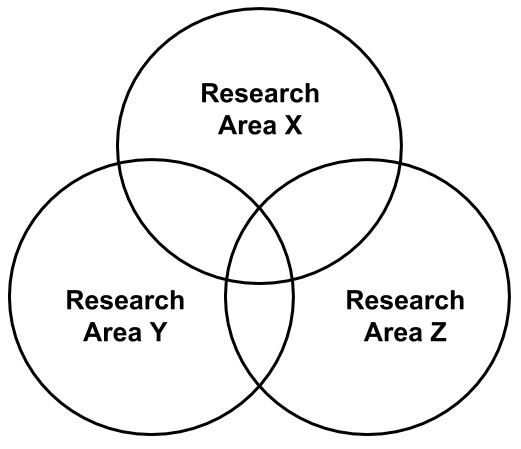
\includegraphics[width=0.5\columnwidth]{research_areas}
    \caption{Research areas}
    \label{fig:research_areas}
\end{figure}


\subsection{Related works}
\label{sub:related_work}

Describe here the contributions and limitations of the related works. It it strongly recommended to construct this section based on a systematic literature review study \cite{kitchenham_2007:systematic_review}.

% ----------
% Hypothesis
\section{Hypothesis}
\label{sec:hypothesis}

This section explains how the proposed research, unlike previous research works, will contribute, with success probabilities, to the solution and comprehension of the stated problem.
% ----------------------
% Research Contributions
\section{Research Contributions}
\label{sec:research_contributions}

This section exposes what are the research and/or innovation contributions of the Master or Doctorate Thesis.

\begin{itemize}
    \item First contribution.
    
    \item Second contribution.
    
    \item Third contribution.
\end{itemize}
% ----------
% Objectives
\section{Objectives}
\label{sec:objectives}

This section must indicate in a very precise way what is the purpose of the work and show a clear and consistent relationship to the problem description and, particularly, to the questions to solve.

It is recommended to formulate a global, general objective, coherent with the stated problem, and two or more specific objectives that will lead to achieving the general objective and that are reachable using the proposed methodology.

The objectives must answer at least one of the following questions: What knowledge is expected to generate? What solution to a specific problem is expected to be achieved from a scientific, technological, and methodological perspective? This is, what is the contribution that will be achieved with the development of the project?

Recall that objectives must not be confused with activities or methodological procedures.

\subsection{General Objective}

Define here the general objective.

\subsection{Specific Objectives}

\begin{itemize}
    \item First specific objective.
    
    \item Second specific objective.
    
    \item Third specific objective.
\end{itemize}
% -----------
% Methodology
\section{Methodology, Activities, and Schedule}
\label{sec:methodology}

\subsection{Methodology}
\label{sub:methodology}

It must be taken into account that the methodological design is the basis for planning all the activities that the project demands and for determining the required human and financial resources.

The activities must correspond to a working methodology and reflect the logical structure of the innovation, research, and development process; these activities must be organized according to the selected methodological approach.

Consequently, the employed methodology must reflect the articulation between the study objectives and the methodological procedures for meeting such objectives. It must be indicated the process to follow for collecting the information as well as the organization, systematization, data analysis, and outcomes presentation.

\subsection{Activities}
\label{sub:activities}

First general activity.

\begin{itemize}
    \item First specific activity of the first general activity.
    
    \item Second specific activity of the first general activity.
    
    \item Third specific activity of the first general activity.
\end{itemize}

Second general activity.

\begin{itemize}
    \item First specific activity of the second general activity.
    
    \item Second specific activity of the second general activity.
    
    \item Third specific activity of the second general activity.
\end{itemize}

\subsection{Schedule}
\label{sub:schedule}

As depicted in Figure \ref{fig:schedule}, the schedule of activities must be presented in a Gantt Diagram that shows the initial date and duration of each one of the general and specific activities.

\begin{figure}[!ht]
    \centering
    \begin{gantt}[xunitlength=0.5cm, fontsize=\scriptsize, titlefontsize=\small, drawledgerline=true]{10}{24}
        \begin{ganttitle}
            \titleelement{Year 1}{12}
            \titleelement{Year 2}{12}
        \end{ganttitle}
        
        \begin{ganttitle}
            \titleelement{Q1}{3}
            \titleelement{Q2}{3}
            \titleelement{Q3}{3}
            \titleelement{Q4}{3}
            \titleelement{Q1}{3}
            \titleelement{Q2}{3}
            \titleelement{Q3}{3}
            \titleelement{Q4}{3}
        \end{ganttitle}
        
        \ganttgroup{\textbf{\footnotesize General Activity A1}}{1}{11}
        \ganttbar{Specific activity A1.1}{1}{3}
        \ganttbar[pattern=crosshatch, color=blue]{Specific activity A1.2}{3}{7}
        \ganttbar[pattern=, fill=gray]{Specific activity A1.3}{8}{4}

        \ganttgroup{\textbf{\footnotesize General Activity A2}}{12}{12}
        \ganttbar[pattern=north east lines, fill=medium-light-gray]{Specific activity A2.1}{12}{4}
        \ganttbarcon[pattern=grid, color=blue, fill=light-gray]{Specific activity A2.2}{16}{4}
        \ganttbarcon[pattern=dots, color=blue, fill=light-gray]{Specific activity A2.3}{20}{4}
    \end{gantt}
    
    \caption{Schedule of activities}
    \label{fig:schedule}
\end{figure}

% ------
% Budget
\section{Budget}
\label{sec:budget}

The budget consists of a summary table with the relationship of the expenses demanded by the development of the project and the financial sources according to the format of Table \ref{tab:budget}.

In case that the project expenses are partially or totally funded by entities or people different from the student(s) and the University that present the proposal, it must be appended the pertinent certifications with the corresponding quantities according to the presented budget, reporting the information in the column \emph{Others}.

\begin{table}[!ht]
    \centering
    \scriptsize
    \begin{tabular}{|l|r|r|r|r|}
        
        \hline
        \multirow{2}{0.2\textwidth}{\centering\textbf{Items}} & \multicolumn{3}{|c|}{\textbf{Sources}} &  \multirow{2}{0.1\textwidth}{\centering\textbf{Total}} \\
        \cline{2-4}
        & \multicolumn{1}{|c|}{\textbf{Student(s)}} & \multicolumn{1}{|c|}{\textbf{FIET}} & \multicolumn{1}{|c|}{\textbf{Others}} & \\
        \hline
        
        \hline
        Human resources & 0.00 & 0.00 & 0.00 & 0.00 \\
        \hline
        Hardware resources & 0.00 & 0.00 & 0.00 & 0.00 \\
        \hline
        Software resources & 0.00 & 0.00 & 0.00 & 0.00 \\
        \hline
        Field trips & 0.00 & 0.00 & 0.00 & 0.00 \\
        \hline
        Resources & 0.00 & 0.00 & 0.00 & 0.00 \\
        \hline
        Various resources & 0.00 & 0.00 & 0.00 & 0.00 \\
        \hline
        Technical services & 0.00 & 0.00 & 0.00 & 0.00 \\
        \hline
        Publications & 0.00 & 0.00 & 0.00 & 0.00 \\
        \hline
        Others & 0.00 & 0.00 & 0.00 & 0.00 \\
        \hline
        \textit{Subtotal} & \textit{0.00} & \textit{0.00} & \textit{0.00} & \textit{0.00} \\
        \hline
        A.U.I. & 0.00 & 0.00 & 0.00 & 0.00 \\
        \hline
        \textbf{Total} & \textbf{0.00} & \textbf{0.00} & \textbf{0.00} & \textbf{0.00} \\
        \hline
        
        \multicolumn{4}{l}{\tiny{\textit{All the values are in COP\$}}}
        
    \end{tabular}
    \caption{Budget}
    \label{tab:budget}
\end{table}

Table \ref{tab:budget_reference} describes the reference criteria for constructing the budget.

\begin{table}[!ht]
    \centering
    \scriptsize
    \begin{tabular}{| p{0.46\textwidth} | p{0.46\textwidth} |}
        
        \hline
        \centertext{\textbf{RESOURCE}} & \centertext{\textbf{REFERENCE VALUE}} \\
        \hline \hline
        
        \multicolumn{2}{|l|}{\textbf{Human resources}} \\
        \hline
        Project advisor &
        Master/Doctorate project: 4 points \\
        \hline
        Research assistant (thesis student, commited 30 hours per week) &
        Master/Doctorate project: 2.5 points \\
        \hline \hline
        
        \multicolumn{2}{|l|}{\textbf{Hardware resources}} \\
        \hline
        Utilization of laboratory equipment: analyzers, measurers, oscilloscopes, development modules, power sources, power strips, etc. &
        25\% of the current market value of the equipment per each 1560 hours of utilization (1 year with 30 hours/week) (4-year depreciation) \\
        \hline
        Printer utilization &
        100\% of the current market value of the printer per each 1000 hours of utilization \\
        \hline
        PC utilization &
        33\% of the current market value of the PC per each 1560 hours of utilization (1 year with 30 hours/week) (3-year depreciation) \\
        \hline
        Others &
        Depends on the particular characteristics \\
        \hline
        All &
        Add a 15\% of the current market value of the hardware resource as a cost for one-year maintenance \\
        \hline \hline
        
        \multicolumn{2}{|l|}{\textbf{Software resources}} \\
        \hline
        Public software utilization &
        No cost \\
        \hline
        Acquisition of specialized tools or bundles &
        Consider a 20\% of the tool acquisition cost \\
        \hline
        Utilization of specialized tools or bundles that have been already acquired &
        \\
        \hline \hline
        
        \multicolumn{2}{|l|}{\textbf{Bibliographic resources}} \\
        \hline
        Documentation &
        Depends on the particular characteristics \\
        \hline
        Data base access &
        Depends on the particular characteristics \\
        \hline \hline
        
        \multicolumn{2}{|l|}{\textbf{Various resources}} \\
        \hline
        Disks, paper, tape &
        Depends on the projected quantity and the current market prices \\
        \hline
        Elements &
        Depends on the specific needs and the respective vendors \\
        \hline
        Communications &
        2\% of the total project value \\
        \hline \hline
        
        \textbf{Technical services} &
        Refers to payment for consulting from external entities \\
        \hline \hline
        
        \multicolumn{2}{|l|}{\textbf{A.U.I.}} \\
        \hline
        This item includes the physical and administrative infrastructure, as well as a backup for unexpected situations &
        20\% of the total project value \\
        \hline
        
    \end{tabular}
    \caption{Reference for budget elaboration}
    \label{tab:budget_reference}
\end{table}
% ----------------
% Submission Terms
\section{Submission Terms}
\label{sec:submission_terms}

This section defines the characteristics and specificities of the products derived from the development of the project.

These products must meet the objectives and specifications demanded in the document of the Master or Doctorate Thesis.

Indicate the minimum number of credits in publications required by the Master or Doctorate program. The final document must append the conducted publications.

\begin{itemize}
    \item First submission term.
    
    \item Second submission term.
    
    \item Third submission term.
\end{itemize}
% ----------
% References
\renewcommand\refname{\vskip -2cm}
\section{References}
\label{references}

Every scientific article or research work that uses theories, data or information from other documents that are considered of great importance for the dealt topic, must be referenced in the work. These references serve to the readers for endorsing what is stated in the work and provide seriousness to the same. Therefore, the proposal of Master or Doctorate Thesis, as well as their final document, must include a well-elaborated bibliographic reference. This part of the proposal Thesis must contain the list of bibliographic references that have been included in the text. Many formats exist, used around the world, that formalize the presentation of the bibliographic references. The Committee suggests using one of the following in the proposal:

\begin{itemize}
    \item IFAC/Elsevier (Harvard): uses the author-date style, \eg (Smith, 1991).
    \item IEEE style: uses an ordered number by the occurrence in the text, \ie [No.]. IEEE is the format style provided in this template.
\end{itemize}

\small
\bibliographystyle{ieeetr}
\bibliography{09-references}
% -------------------------------
% Intellectual Property Agreement
\makeagreement
% ------------
\end{document}
